\documentclass{article}
\usepackage{tikz}
\usetikzlibrary{positioning} %for node positioning using name
\title{Baiscs(From Overleaf)}
\author{Sumaiya Tabassum}
\begin{document}
	\maketitle
	\tableofcontents
	\clearpage
	
	\section{Intersection Point}
	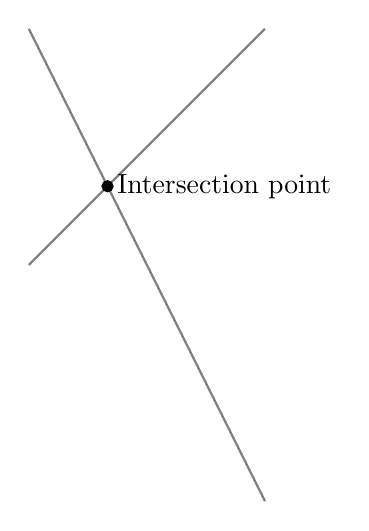
\begin{tikzpicture}
		\draw[gray, thick] (-1,2) -- (2,-4);
		\draw[gray, thick] (-1,-1) -- (2,2);
		\filldraw[black] (0,0) circle(2pt)
				 node[anchor = west]
				 {Intersection point};
	\end{tikzpicture}
	
	\section{Points, Lines and Paths}
	\begin{tikzpicture}
		\draw (-2,0) -- (2,0);
		\filldraw [gray] (0,0) circle (2pt);
		\draw (-2,-2) .. controls (0,0) .. (2,-2); %Draws a Bézier curve, one control point
		\draw (-2,2) .. controls (-1,0) and (1,0) .. (2,2); %Draws a Bézier curve, two control point
	\end{tikzpicture}
	
	\section{Basic Geometric Shapes}
	\begin{minipage}{0.25\textwidth}	
		\subsection{Circle}
		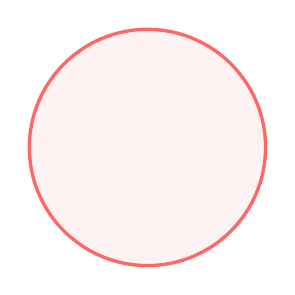
\begin{tikzpicture}
			\filldraw[color=red!60, fill=red!5, very thick] (-1,0) circle(1.5);
		\end{tikzpicture}
	\end{minipage}
	\hfill
	\begin{minipage}{0.25\textwidth}	
		\subsection{Ellipse}
		
\begin{tikzpicture}
			\fill[blue!50] (2.5,0) ellipse (1.5 and 0.5);
		\end{tikzpicture}
	\end{minipage}
	\hfill
	\begin{minipage}{0.25\textwidth}	
		\subsection{Arc}
		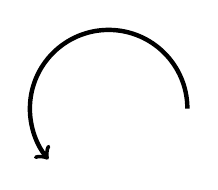
\begin{tikzpicture}
			\draw[ultra thick, ->] (6.5,0) arc (0:220:1);
		\end{tikzpicture}
	\end{minipage}
	
	\section{Polygons}
	\begin{minipage}{0.45\textwidth}
	\subsection{Square}
		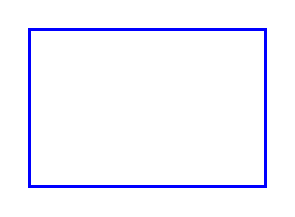
\begin{tikzpicture}
			\draw[blue, very thick] (0,0) rectangle (3,2);
		\end{tikzpicture}
	\end{minipage}
	\hfill
	\begin{minipage}{0.45\textwidth}	
		\subsection{Triangle}
		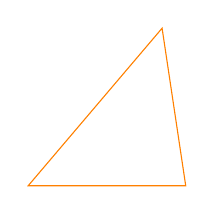
\begin{tikzpicture}
			\draw[orange] (4,0) -- (6,0) -- (5.7,2) -- cycle;
		\end{tikzpicture}
	\end{minipage}
	
	\section{Diagrams}
	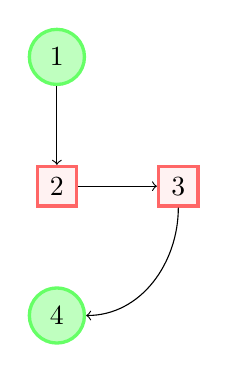
\begin{tikzpicture}
		[roundnode/.style={circle,draw=green!60, fill=green!25,very thick, minimum size=7mm},
		squarenode/.style={rectangle, draw=red!60, fill=red!5,very thick, minimum size=5mm},
		]
		
		%Nodes
		\node[squarenode](maintopic){2};
		\node[roundnode](uppercircle)[above=of maintopic] {1};
		\node[squarenode](rightsquare)[right=of maintopic] {3};
		\node[roundnode](lowercircle)[below=of maintopic] {4};
		%Lines
		\draw[->](uppercircle.south) -- (maintopic.north);
		\draw[->](maintopic.east) -- (rightsquare.west);
		\draw[->](rightsquare.south) .. controls +(down:7mm) and + (right:7mm) .. (lowercircle.east);
	\end{tikzpicture}
\end{document}